% docs/dissertation/tex/secao_6_8_sinal_da_covariancia.tex
% Seção 6.8 do capítulo clínico — "O sinal da covariância decide o dano" (RQ4, 2026-08-31).
% Pronta para \input{} num documento que carregue graphicx, amsmath e babel/polyglossia pt-BR.
% Figura: docs/dissertation/figures/fig_rq4_flip_rate_2026-08-31.{svg,png} (PNG 1800 px para LaTeX).
% Fonte dos números: docs/research/sounio/rq4_vanco_two_compartment_flip.sio e
% rq4_vanco_mc_adequacy.sio (Madaros committed; determinísticos; linhas RQ4_FLIP / RQ4_MC).

\section{O sinal da covariância decide o dano}
\label{sec:sinal-covariancia}

Toda biblioteca de propagação de incerteza que a farmacometria usa --- e o
\texttt{ep\_add}/\texttt{ep\_mul} do próprio \texttt{stdlib/epistemic/knowledge} ---
assume que os operandos de cada operação são independentes. Numa cadeia farmacocinética
essa hipótese é falsa por construção: peso, creatinina e depuração entram mais de uma vez,
e cada reencontro carrega uma covariância que a biblioteca omite. Pelo Lema~1 da
formalização (\texttt{trueVar\_append} em \texttt{EpistemicEffectsNS.lean}), a variância
reportada erra exatamente em $2\,\mathrm{Cov}$; o que não se sabia era quanto disso chega a
uma decisão clínica.

Medimos isso numa coorte determinística de $5\,000$ pacientes (peso 45--120~kg,
creatinina 0,6--2,6~mg/dL, $Q$ e $V_p$ a $\pm 30\,\%$ da população; 500~mg a cada 12~h),
com a regra de decisão do exemplo canônico --- \textsc{warn} quando a estimativa pontual
de $\mathrm{AUC}_{0\text{--}24}$ é terapêutica ($\geq 400$~mg$\cdot$h/L) mas o limite
inferior do IC95 cruza os 400 --- propagada de três formas: formas afins de primeira ordem
que rastreiam as fontes de medição (a verdade, a mesma construção \texttt{Aff} do cálculo
mecanizado em Lean), a cadeia escalar \texttt{ep\_*} como é (independência em toda
operação) e operandos exatos com uma única adição final independente, que isola o termo
$2\,\mathrm{Cov}$.

Em duas somas de fontes compartilhadas que um software de TDM realmente executa, o
resultado tem os dois sinais (Figura~\ref{fig:rq4-flip}). Na soma de intervalos
$\mathrm{AUC}(0\text{--}12) + \mathrm{AUC}(12\text{--}24)$, ambos derivados da mesma
depuração ($\rho = 1$), a adição ingênua reduz a variância exatamente à metade --- a
contração de $\sqrt{2}$ no desvio-padrão --- e \textbf{silencia 311 dos 909 \textsc{warn}s
verdadeiros (34,2\,\%)}: um alerta em três desaparece, e o paciente lê ``terapêutico''.
Na decomposição da AUC em fases, $A/\alpha + B/\beta$, a covariância entre as fases é
\textbf{negativa em 5\,000 de 5\,000 pacientes} --- porque a AUC é invariante a $Q$ e $V_p$
e a decomposição é uma partição desse invariante: o que $Q$ e $V_p$ movem para uma fase
retiram da outra, agora um teorema do cálculo (\texttt{inner\_nonpos\_of\_partition}: toda
fonte de partição contribui $-(\partial a/\partial\varepsilon)^2 \leq 0$ à covariância)
--- e a mesma hipótese de independência erra na direção oposta: sobrestima a variância em
20\,\% na soma final e em \textbf{300 vezes} ao longo da cadeia inteira, produzindo
\textbf{1\,894 \textsc{warn}s espúrios (38\,\% da coorte)} e silenciando nenhum. É o outro
dano clínico, a fadiga de alarme, produzido pelo mesmo defeito.

O sinal da covariância decide qual dano se obtém; o compilador não precisa conhecê-lo. A
disciplina de conjuntos de fontes (E230) recusa a adição com fontes compartilhadas nos dois
casos, e a propagação afim (\texttt{stdlib/epistemic/affine}) computa a soma correta nos
dois --- o que o teorema \texttt{naive\_add\_understates\_iff} (anti-\emph{garbling}
$\Leftrightarrow \mathrm{Cov} > 0$) e seus corolários enunciam, e o que a coorte confirma:
sob a propagação exata, os 909 alertas são exatamente os 909 que deveriam existir. E a
verdade de primeira ordem é a verdade de amostragem: uma Monte Carlo da mesma coorte
($1\,000$ sorteios por paciente) reproduz a variância afim em 0,1\,\% em média (razão
0,999; extremos 0,857 e 1,158 na cauda de baixa depuração) e a mesma decisão de \textsc{warn}
em 99,4\,\% dos pacientes, ao custo $O(N_p)$ de uma única propagação em vez de $10^6$
avaliações --- e confirma que a sobrestimação de 300 vezes da cadeia ingênua é real contra
a amostragem (300,9), não um artefato da linearização.

\begin{figure}[htbp]
  \centering
  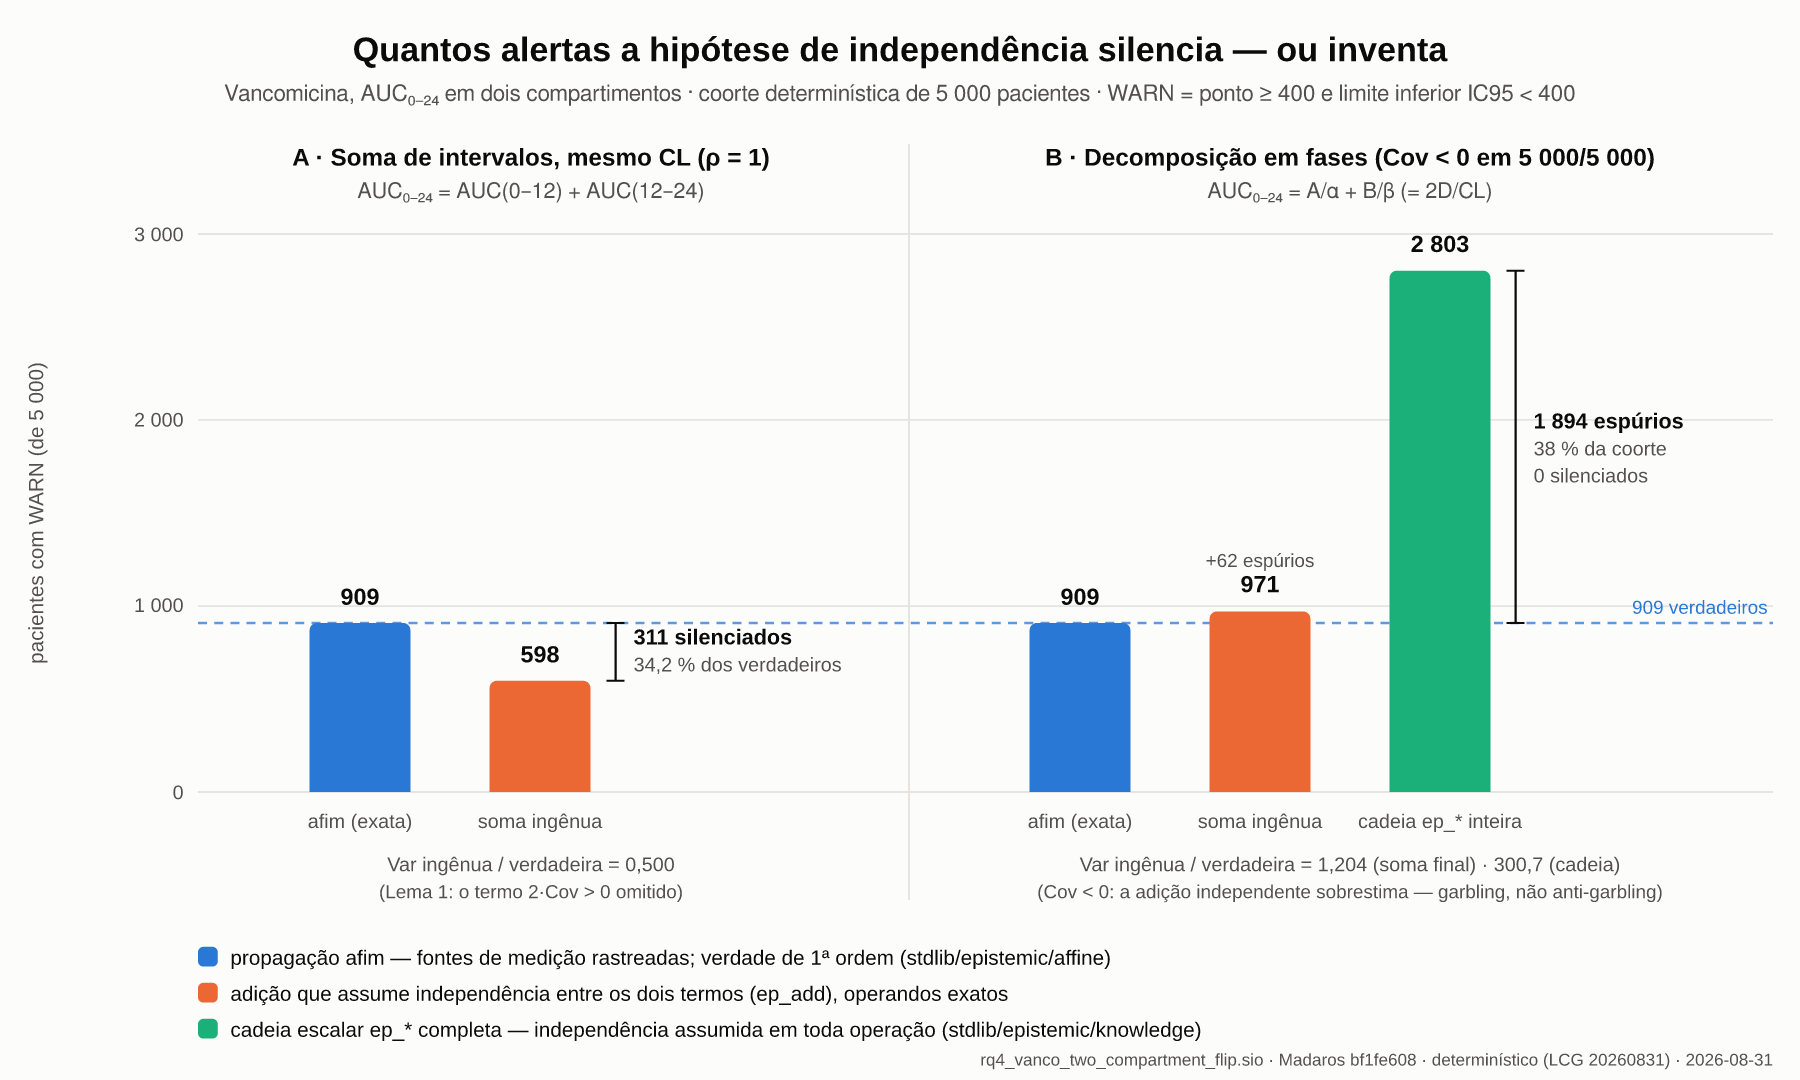
\includegraphics[width=\textwidth]{figures/fig_rq4_flip_rate_2026-08-31.png}
  \caption[Quantos alertas a hipótese de independência silencia --- ou inventa]{%
    \textbf{Quantos alertas a hipótese de independência silencia --- ou inventa.}
    Coorte determinística de $5\,000$ pacientes; $\mathrm{AUC}_{0\text{--}24}$ de
    vancomicina em dois compartimentos; \textsc{warn} = estimativa pontual
    $\geq 400$~mg$\cdot$h/L e limite inferior do IC95 $< 400$. A propagação afim (fontes
    de medição rastreadas; verdade de 1ª ordem) produz 909 \textsc{warn}s, a linha
    tracejada. \textbf{(A)} Soma de intervalos $\mathrm{AUC}(0\text{--}12) +
    \mathrm{AUC}(12\text{--}24)$ a partir da mesma depuração ($\rho = 1$): a adição que
    assume independência reporta metade da variância (razão 0,500; Lema~1 com o termo
    $2\,\mathrm{Cov} > 0$ omitido) e silencia 311 \textsc{warn}s (34,2\,\%).
    \textbf{(B)} Decomposição em fases $A/\alpha + B/\beta = 2D/\mathrm{CL}$: a
    covariância entre as fases é negativa em todos os pacientes, a adição independente
    sobrestima (razão 1,204; +62 \textsc{warn}s espúrios) e a cadeia escalar
    \texttt{ep\_*} completa sobrestima 300 vezes (2\,803 \textsc{warn}s; 1\,894 espúrios,
    38\,\% da coorte; nenhum silenciado). Programa
    \texttt{rq4\_vanco\_two\_compartment\_flip.sio}, Madaros committed, 2026-08-31;
    identidade $A/\alpha + B/\beta = 2D/\mathrm{CL}$ verificada a erro zero em primeira
    ordem.}
  \label{fig:rq4-flip}
\end{figure}
